%%%%%%%%%%%%%%%%%%%%%%%%%%%%%%%%%%%%%%%%%
% baposter Landscape Poster
% LaTeX Template
% Version 1.0 (11/06/13)
%
% baposter Class Created by:
% Brian Amberg (baposter@brian-amberg.de)
%
%
% License:
% CC BY-NC-SA 3.0 (http://creativecommons.org/licenses/by-nc-sa/3.0/)
%
%%%%%%%%%%%%%%%%%%%%%%%%%%%%%%%%%%%%%%%%%

%----------------------------------------------------------------------------------------
%PACKAGES AND OTHER DOCUMENT CONFIGURATIONS
%----------------------------------------------------------------------------------------

\documentclass[landscape,a0paper,fontscale=0.33]{baposter} % Adjust the font scale/size here

\usepackage{graphicx} % Required for including images
\graphicspath{{figures/}} % Directory in which figures are stored

\usepackage{amsmath} % For typesetting math
\usepackage{amssymb} % Adds new symbols to be used in math mode

\usepackage{booktabs} % Top and bottom rules for tables
\usepackage{enumitem} % Used to reduce itemize/enumerate spacing
\usepackage[font=small,labelfont=bf]{caption} % Required for specifying captions to tables and figures
\usepackage{tcolorbox}
\usepackage{listings}
\usepackage{multicol} % Required for multiple columns
\setlength{\columnsep}{1.5em} % Slightly increase the space between columns
\setlength{\columnseprule}{0mm} % No horizontal rule between columns
\usepackage[T1]{fontenc}
\usepackage{tikz} % Required for flow chart
\usetikzlibrary{shapes,arrows} % Tikz libraries required for the flow chart in the template
\usepackage{fix-cm}
\newcommand{\compresslist}{ % Define a command to reduce spacing within itemize/enumerate environments, this is used right after \begin{itemize} or \begin{enumerate}
\setlength{\itemsep}{1pt}
\setlength{\parskip}{0pt}
\setlength{\parsep}{0pt}
}

\definecolor{lightblue}{rgb}{.54,.824,1.} % Defines the color used for content box headers
\definecolor{whiteblue}{RGB}{240,255,255} % Defines the color used for content box headers

\begin{document}

\begin{poster}
{
headershade=plain,
headerborder=closed, % Adds a border around the header of content boxes
colspacing=1em, % Column spacing
bgColorOne=white, % Background color for the gradient on the left side of the poster
bgColorTwo=white, % Background color for the gradient on the right side of the poster
borderColor=lightblue, % Border color
headerColorOne=blue, % Background color for the header in the content boxes (left side)
headerColorTwo=blue, % Background color for the header in the content boxes (right side)
headerFontColor=white, % Text color for the header text in the content boxes
boxColorOne=lightblue, % Background color of the content boxes
textborder=rounded, % Format of the border around content boxes, can be: none, bars, coils, triangles, rectangle, rounded, roundedsmall, roundedright or faded
eyecatcher=true, % Set to false for ignoring the left logo in the title and move the title left
headerheight=0.\textheight, % Height of the header
headershape=rounded, % Specify the rounded corner in the content box headers, can be: rectangle, small-rounded, roundedright, roundedleft or rounded
headerfont=\Large\bf\textsf, % Large, bold and sans serif font in the headers of content boxes
%textfont={\setlength{\parindent}{1.5em}}, % Uncomment for paragraph indentation
linewidth=2pt, % Width of the border lines around content boxes
columns=3
}
%----------------------------------------------------------------------------------------
%TITLE SECTION 
%----------------------------------------------------------------------------------------
%
{} % First university/lab logo on the left
{} % Poster title
{} % Author names and institution
{} % Second university/lab logo on the right

%----------------------------------------------------------------------------------------
%RooFit, RooStats and HistFactory
%----------------------------------------------------------------------------------------
\sffamily
\headerbox{}{name=intro,column=0,row=0,headerborder=none,textborder=none,headerColorOne=white,headershade=plain,boxColorOne=white}{
\begin{center}{\textcolor{lightblue}{\textbf{\fontsize{30}{30}\selectfont RooFit \& RooStats}}}

{\Large a python data science{\it Cheat Sheet}}\end{center}
%\vspace{0.5em} % When there are two boxes, some whitespace may need to be added if the one on the right has more content
}

%----------------------------------------------------------------------------------------
%CONTACT INFORMATION
%----------------------------------------------------------------------------------------

\headerbox{Contact Information}{name=contact,column=2,above=bottom}{ % This block is as tall as the references block

\begin{description}\compresslist
\item[Web] www.university.edu/smithlab
\item[Email] john@smith.com
\item[Phone] +1 (000) 111 1111
\end{description}
}

%----------------------------------------------------------------------------------------
%About RooFit
%----------------------------------------------------------------------------------------

\headerbox{What is RooFit?}{name=about,column=0,below=intro}{ % This block's bottom aligns with the bottom of the conclusion block

The Toolkit for Data Modeling with \textbf{\tt ROOT} ({\bf RooFit}) is a package that allows for modeling probability distributions in a compact and abstract way. {\bf RooStats} is a project to create statistical tools built on top of {\bf RooFit} and distributed in \textbf{\tt ROOT}. It is a joint project between the LHC experiments and the \textbf{\tt ROOT} team.

\begin{tcolorbox}[colback=blue!5!white,colframe=blue!75!black,title=A Simple Example]
\tt{
import ROOT\\
w = ROOT.RooWorkspace()\\
w.factory('Gaussian::g(x[-5,5],mu[-3,3],sigma[1])')\\
w.factory('Exponential::e(x,tau[-.5,-3,0])')\\
w.factory('SUM::model(s[50,0,100]*g,b[100,0,1000]*e)')\\
x = w.var('x')\\
pdf = w.pdf('model')\\
frame = x.frame()\\
data = pdf.generate(ROOT.RooArgSet(x))\\
data.plotOn(frame)\\
fitResult = pdf.fitTo(data,ROOT.RooFit.Save())\\
pdf.plotOn(frame)\\
frame.Draw()\\
}
\begin{center}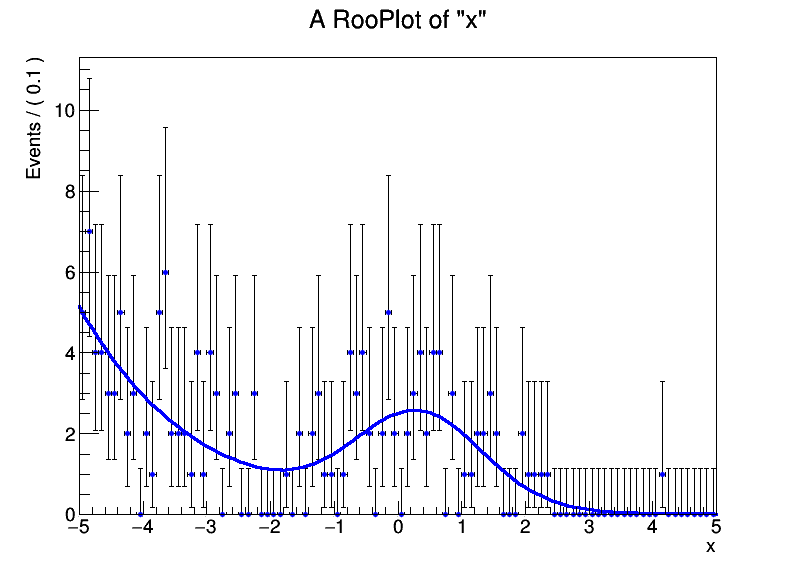
\includegraphics[width=0.75\linewidth]{simpleexample01}\end{center}
\end{tcolorbox}
}


%----------------------------------------------------------------------------------------
%Histfactory
%----------------------------------------------------------------------------------------

\headerbox{Statistical Tests with RooStats}{name=tests,column=2,span=1,row=0,bottomaligned=about}{


}



%----------------------------------------------------------------------------------------
%Fitting
%----------------------------------------------------------------------------------------

\headerbox{Parameter Estimation and Fitting}{name=fitting,column=1}{ % This block's bottom aligns with the bottom of the conclusion block

The following materials were required to complete the research:

\begin{itemize}\compresslist
\item Curabitur pellentesque dignissim
\item Eu facilisis est tempus quis
\item Duis porta consequat lorem
\item Eu facilisis est tempus quis
\end{itemize}

The following equations were used for statistical analysis:
}

%----------------------------------------------------------------------------------------
%RooFit Data types
%----------------------------------------------------------------------------------------

\headerbox{RooVariables, RooPdfs, Data and Composite Models}{name=vars,column=0,span=3,below=about,above=bottom}{ % This block's bottom aligns with the bottom of the conclusion block

\begin{multicols}{3}
RooFit classes have a 1:1 correspondences to mathematical objects. e.g. variable $\rightarrow$ RooRealVar, function $\rightarrow$ RooAbsReal, probability density function $\rightarrow$ RooAbsPdf.\\
\begin{tcolorbox}[colback=blue!5!white,colframe=blue!75!black,width=1.03\linewidth,title=Variables and P.D.Fs]
\tt{
observable = ROOT.RooRealVar(``x'',''x'',-10,10)\\
mean = ROOT.RooRealVar(``mean'',''Mean'',-10,10)\\
sigma = ROOT.RooRealVar(``sigma'',''Width'',3,-10,10)\\
gauss = ROOT.RooGaussian(``gauss'',''pdf title'',x,mean,sigma)
}
\end{tcolorbox}
\begin{tcolorbox}[colback=blue!5!white,colframe=blue!75!black,width=1.03\linewidth,title=Importing Data from Histograms]
\tt{
hh = ROOT.TH1F(``hh'',''some histogram'',21,-10,10)\\
x = ROOT.RooRealVar(``x'',''x'',-10,10)\\
data = ROOT.RooDataHist(``data'',''dataset with x'',x,hh)}
\end{tcolorbox}

\columnbreak

\begin{tcolorbox}[width=2.05\linewidth,colback=blue!5!white,colframe=blue!75!black,title=Common P.D.Fs]
\begin{tabular}{l | l c}
\tt{ROOT.RooBifurGauss(``name'', ``title'', $x$, $\mu$, $\sigma_L$, $\sigma_R$)} & Bifurcated Gaussian & $f(x;\mu,\sigma)=\frac{1}{N}\cdot \exp(-(x-\mu)^2/(2\sigma(x-\mu)^2)$\\
\tt{ROOT.RooExponential(``name'', ``title'', $x$, $c$)} & Exponential & $f(x;c)=\frac{1}{N}\exp (c x)$\\
\tt{ROOT.RooPolynomial(``name'', ``title'', $x$, RooArgList($c_1$,$c_2$)} & Polynomial & $f(x;c_0,...,c_n)=\frac{1}{N}\cdot\left(1+\sum_{k=1}^{n}c_kx^k\right)$\\
\tt{ROOT.RooPoisson(``name'', ``title'', $x$, $\eta$)} & Poisson & $f(x;\eta)=\frac{1}{x!}\cdot\eta^x\exp(-\eta)$
\end{tabular}
\end{tcolorbox}
\begin{tcolorbox}[colback=blue!5!white,colframe=blue!75!black,width=1.03\linewidth,title=Composite Models from P.D.Fs]
For a set of PDFs e.g. \tt{signalpdf} and \tt{backgroundpdf} and a fractional normalization \tt{fsig}:\\
\tt{
fsig = ROOT.RooRealVar(``fsig'',''signal fraction'',0.5,0.,1.)\\
model = ROOT.RooAddPdf(``model'',''model'',\\
\hspace*{2cm}RooArgList(signalpdf,backgroundpdf),RooArgList(fsig))
}
\end{tcolorbox}

\columnbreak
\vspace*{3cm}
Some text here. Explaining caveats or links to more PDFs etc.\\

Possible location for ROOT, RooFit, DIANA-hep and NIKHEF logos. 
\columnbreak


\end{multicols}
}


%----------------------------------------------------------------------------------------
%Workspaces
%----------------------------------------------------------------------------------------

\headerbox{Working with workspaces}{name=workspaces,column=1,below=fitting,bottomaligned=about}{ % This block's bottom aligns with the bottom of the conclusion block

The following materials were required to complete the research:

\begin{itemize}\compresslist
\item Curabitur pellentesque dignissim
\item Eu facilisis est tempus quis
\item Duis porta consequat lorem
\item Eu facilisis est tempus quis
\end{itemize}

The following equations were used for statistical analysis:
}



%----------------------------------------------------------------------------------------

\end{poster}

\end{document}
